\documentclass[12pt]{article}
\usepackage[utf8]{inputenc}
% \usepackage{margin=1in}{geometry}
\usepackage{setspace}
\usepackage{harvard}
\usepackage{graphicx}
\usepackage[style=authoryear]{biblatex}
\addbibresource{bib.bib}

\begin{document}

\title{LSTMs for Semi-Supervised Text Classification}
\author{Abhay}
\date{}
\maketitle
\singlespacing

\begin{abstract}
    The following document describes in brief the model by \cite{sachan2019revisiting}. It suggests very simple and robust approach for the task of text classification with both supervised and semi-supervised approaches. On contrary to the complex schemes and models suggested by various researches, this model is based on a simple BiLSTM model, trained with cross-entropy loss. Also, this incorporates the use of various losses via mixed objective function and is able to  produce state of the art results for text classification tasks.
\end{abstract}
\section{Introduction}
    Text classification also known as text tagging or text categorization is the process of categorizing text into organized groups. Text Classification has always been a defining problem in the field of natural language processing. It covers a very broad area of NLP in terms of  applications like sentiment analysis, email filtering, language detection and many more.
    Earliest approaches were based on the extraction of bag of words features followed by either Naive Byes(\cite{mccallum1998comparison}) or linear SVM (\cite{joachims1998text}). Recently, RNN and CNN models were introduced to utilize the word order and grammatical structure as shown by \cite{kim2014convolutional}. The previous state of the art techniques either use pretrained LSTMs or complex computationally expensive model.
    This model proposes a mixed objective function for semi supervised learning without the requirement of any pretraining step.
\section{Details}
\subsection{Model Architecture}
The Figure \ref{fig:model} represent the classification model

\begin{figure}
    % \centering
    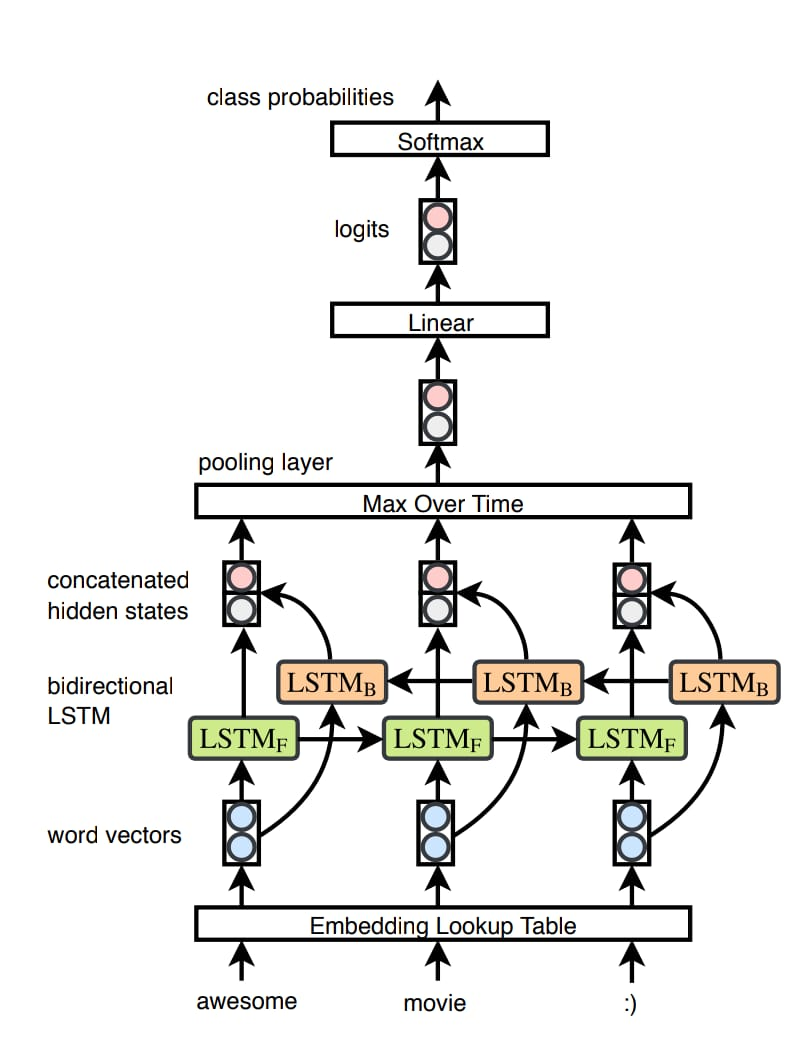
\includegraphics[width=0.6\linewidth]{Model.jpeg}    
    \caption{Model}
    \label{fig:model}
\end{figure}
\subsection{Methods}
\subsubsection{Supervised training}
Let there be $m$ labeled examples in the training set that
are denoted as ${(x^{(1)} , y^{(1)} ), . . . , (x^{(m)} , y^{(m)} )}$, where $x^{(i)}$
represents a document’s word sequence, $y^{(i)}$ represents class
label such that $y^{(i)} \in  (1, 2, . . . , K)$. For supervised training
of the classification model, we make use of two methodologies: maximum likelihood estimation and adversarial training:-
\begin{equation}
    \label{eq:Ml}
    L_{ML}(\theta) = -1/m_{l} * \sum^{m_{l}}_{i=1} \sum^{K}_{j=1} z (y^{(i)} = k) log p(y^{i}= k |x^{i};\hat{\theta})
\end{equation}
\begin{equation}
    \label{eq:AT}
    L_{AT}(\theta) = -1/m_{l} * \sum^{m_{l}}_{i=1} \sum^{K}_{k=1} z (y^{(i)} = k) log p(y^{i}= k |v^*{i};\hat{\theta})
\end{equation}
where $v^{*}$ corresponds to adversarial embedding corresponding to v
\subsubsection{Unsupervised Training}
The model also uses experiments two unsupervised methods like Virtual Adversarial training and Entropy Minimization.
\begin{equation}
    \label{eq:AT}
    L_{EM}(\theta) = -1/m * \sum^{m}_{i=1} \sum^{K}_{k=1}p(y^{(i)} = k|x^{(i)}) log p(y^{i}= k |x^({i}))
\end{equation}
where $m=m_{l}+m_{u}$ and dependence on $\theta$ is suppressed
\begin{equation}
    \label{eq:Vat}
    L_{VAT}(\theta)= 1/m * \sum^{m}_{i=1} D_{KL}(p(.|v^{(i)};\theta)||p(.|v^{(*i)};\theta)
\end{equation}
where $m= m_{l} + m_{u}$
\subsubsection{Mixed Objective Function}
Thus the proposed mixed objective function using $\lambda_{ML}$, $\lambda_{AT}$, $\lambda_{EM}$ and $\lambda_{VAT}$ as parameters become 
\begin{equation}
    L_{mixed}= \lambda_{ML}L_{ML} + \lambda_{VAT}L_{AT} + \lambda_{EM}L_{EM} + \lambda_{VAT}L_{VAT} 
\end{equation}
\subsection{Results}
The model was experimented with the datasets shown in Table \ref{tab:dataset}
\begin{table}[]
    
    \begin{tabular}{|c|c|c|c|c|}
        \hline
        Dataset & Train & Test & K & L\\
        \hline
        ACL IMDB & 25000 & 25000 & 2 & 268\\  
        Elec & 25000 & 25000 & 2 & 125\\
        AG-News & 120,000 & 7,600 & 4 & 46\\
        \hline
    \end{tabular}
    \caption{Summary statistics for text classification datasets;
K = number of classes; L = average length of a document.}
    \label{tab:dataset}
\end{table}
The error rates (\%) when model is trained using mixed objective functon are shown in Table \ref{tab:results}

\begin{table}[]
    \begin{tabular}{|c|c|c|c|}
        \hline
        Model & ACl IMDB & Elec & AG-News\\
        \hline
        LSTM & 5.91 & 5.40 & 6.78 \\
        oh-LSTM & 5.94 & 5.55 & 6.57 \\
        ULMFit & 4.60 & - & 5.01 \\
        \hline
        $L_{Mixed}$ & 4.32 & 5.24 & 4.9\\
        \hline
    \end{tabular}
    \caption{Error rates (\%) of $L_{Mixed}$ compared with previous best methods}
    \label{tab:results}
\end{table}

\section{Conclusion}
\cite{sachan2019revisiting} has shown that a simple BiLSTM model using a combination of various loss functions reported state of the art performance on several text classification datasets and the mixed objective function can be generalise to other tasks such as relation extraction.
\printbibliography
\end{document}
